\documentclass{report}
%\usepackage{tikz}
%& -shell-escape
\usepackage{pgfplots}
\pgfplotsset{compat=newest}

\usepackage{tkz-fct}
\usetkzobj{all}
\begin{document}
	
%\begin{center}
%\begin{figure}
%	\begin{minipage}{0.70\linewidth}
%		\includegraphics[width=1\linewidth]{imageEPS.eps}
%		\caption{Problème industriel}
%	\end{minipage}
%\end{figure}
%\end{center}
\section{A}
		\input |"ls *.tex"
\section{B}


\begin{figure}
\centering
\resizebox {12cm} {!} {
	\input |"sed -e 's/width=[0-9]*.[0-9]*in,/width=9cm,/' CalculSchem3.T2.tikz > CalculSchem3.T2.tikzb"
	\input |"sed -e 's/height=[0-9]*.[0-9]*in,/height=6cm,/' CalculSchem3.T2.tikzb > CalculSchem3.T2.tikzc"
		% This file was created by matlab2tikz v0.4.7 (commit 9d7ddd53b3fb1f0df255c7d242269793e3f459e5) running on MATLAB 7.14.
% Copyright (c) 2008--2014, Nico Schlömer <nico.schloemer@gmail.com>
% All rights reserved.
% Minimal pgfplots version: 1.3
% 
% The latest updates can be retrieved from
%   http://www.mathworks.com/matlabcentral/fileexchange/22022-matlab2tikz
% where you can also make suggestions and rate matlab2tikz.
% 

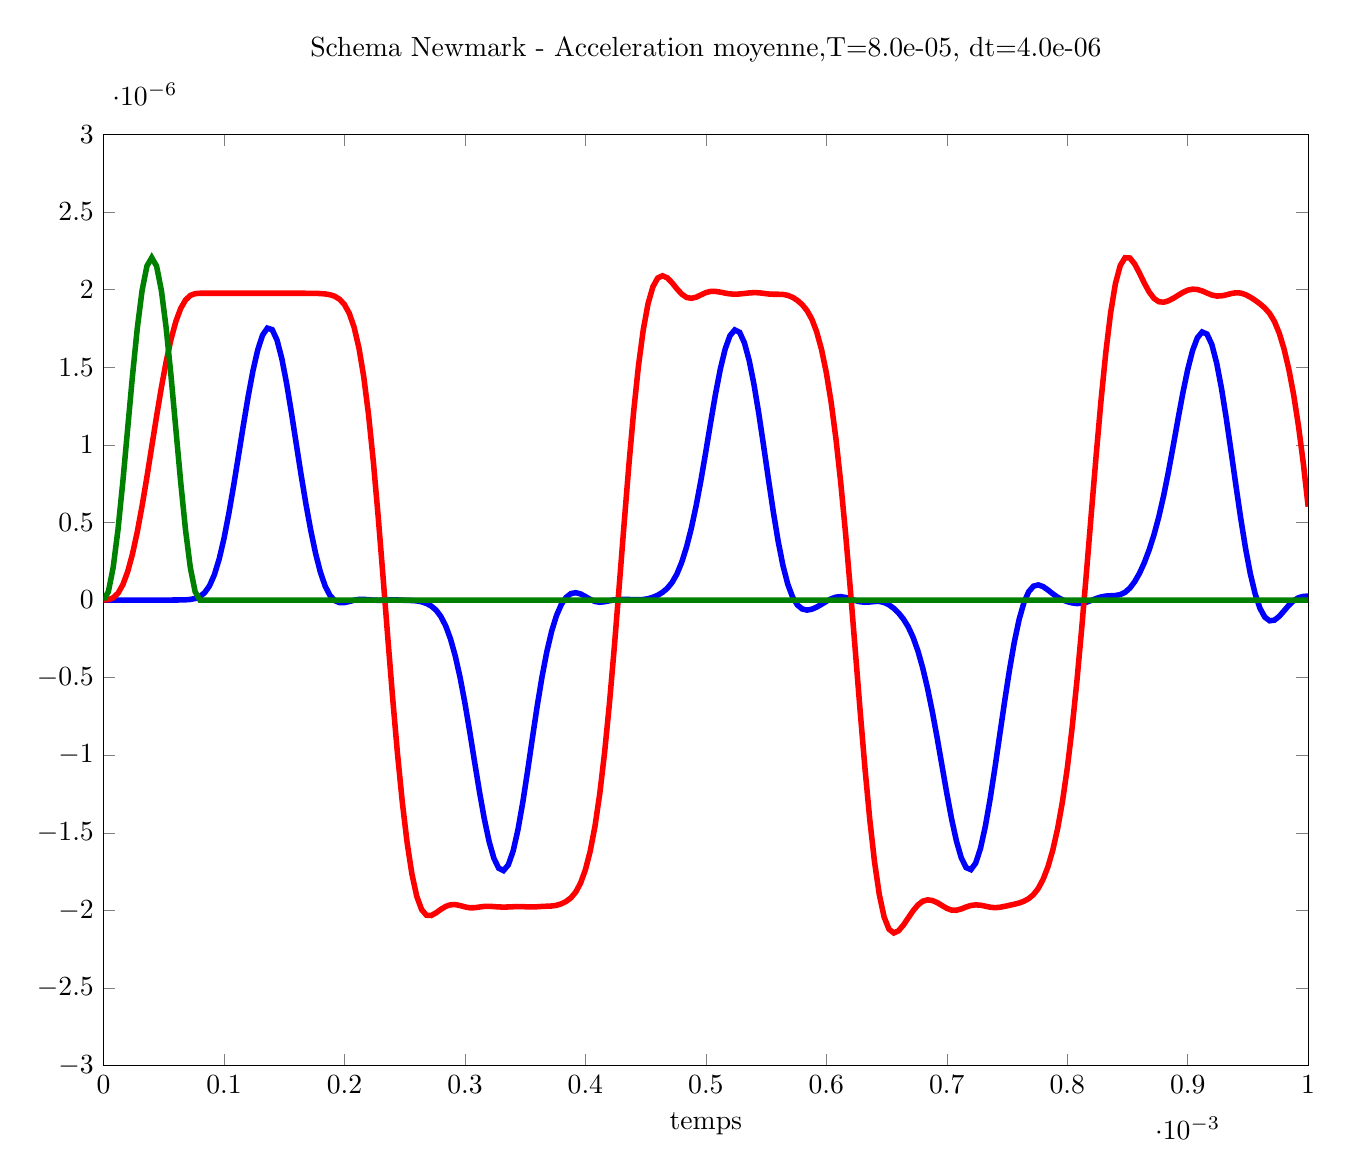
\begin{tikzpicture}{scale=10}

\begin{axis}[%
title={\centering Schema Newmark - Acceleration moyenne,\newline T=8.0e-05, dt=4.0e-06},
%title style={text width=9cm},
title style={at={(0.5,1.05)}},
width=6.02303149606299in,
height=4.6560531496063in,
scale only axis,
scale=1,
xmin=0,
xmax=0.001,
ymin=-3e-06,
ymax=3e-06,
xlabel=temps,
%grid=major,
]

\addplot [color=blue,solid,line width=2.0pt,forget plot]
  table[row sep=crcr]{0	0\\
4e-06	3.14139442609617e-25\\
8e-06	2.50153862049487e-23\\
1.2e-05	9.72557197161409e-22\\
1.6e-05	2.4595713633591e-20\\
2e-05	4.54827407088953e-19\\
2.4e-05	6.55446993403166e-18\\
2.8e-05	7.6607181450013e-17\\
3.2e-05	7.46207899980209e-16\\
3.6e-05	6.17759444632606e-15\\
4e-05	4.41077313521841e-14\\
4.4e-05	2.7468690146802e-13\\
4.8e-05	1.50528989066344e-12\\
5.2e-05	7.30972473234866e-12\\
5.6e-05	3.16310585891182e-11\\
6e-05	1.22523040085308e-10\\
6.4e-05	4.26383503695668e-10\\
6.8e-05	1.33708856275083e-09\\
7.2e-05	3.78776695617489e-09\\
7.6e-05	9.71453192193973e-09\\
8e-05	2.26039725574304e-08\\
8.4e-05	4.78243723489142e-08\\
8.8e-05	9.22580659820298e-08\\
9.2e-05	1.62864697242951e-07\\
9.6e-05	2.64409565414341e-07\\
0.0001	3.97429926476515e-07\\
0.000104	5.57770455712265e-07\\
0.000108	7.38027973099106e-07\\
0.000112	9.29593109425346e-07\\
0.000116	1.1234622171808e-06\\
0.00012	1.3095804134545e-06\\
0.000124	1.47643697282926e-06\\
0.000128	1.61225353624043e-06\\
0.000132	1.70676278411038e-06\\
0.000136	1.7518893076128e-06\\
0.00014	1.74189541185508e-06\\
0.000144	1.67488609706296e-06\\
0.000148	1.55516494038599e-06\\
0.000152	1.39357676233087e-06\\
0.000156	1.20491291884901e-06\\
0.00016	1.00453934769113e-06\\
0.000164	8.0586442790366e-07\\
0.000168	6.18614123404745e-07\\
0.000172	4.48758911453188e-07\\
0.000176	3.00768000293816e-07\\
0.00018	1.79507796910571e-07\\
0.000184	8.88578913684288e-08\\
0.000188	2.89764193277664e-08\\
0.000192	-4.13007375106895e-09\\
0.000196	-1.69063012724583e-08\\
0.0002	-1.64856265714507e-08\\
0.000204	-9.44506864240009e-09\\
0.000208	-1.25474440559732e-09\\
0.000212	3.92276495690471e-09\\
0.000216	4.38504461366123e-09\\
0.00022	1.80721720397064e-09\\
0.000224	-7.37185377446172e-10\\
0.000228	-1.70197812671894e-09\\
0.000232	-1.22319617393971e-09\\
0.000236	3.53085090533751e-11\\
0.00024	9.34884033824151e-10\\
0.000244	4.32199165469258e-10\\
0.000248	-1.06357523759277e-09\\
0.000252	-2.26768897250803e-09\\
0.000256	-3.17355896065272e-09\\
0.00026	-5.57276887478506e-09\\
0.000264	-1.14202551064067e-08\\
0.000268	-2.18251274996877e-08\\
0.000272	-3.84334986087291e-08\\
0.000276	-6.48884822511927e-08\\
0.00028	-1.05943306819033e-07\\
0.000284	-1.6626377503046e-07\\
0.000288	-2.50319236554444e-07\\
0.000292	-3.6134764835012e-07\\
0.000296	-5.00082806852344e-07\\
0.0003	-6.64560869812467e-07\\
0.000304	-8.48886678560027e-07\\
0.000308	-1.04243179208542e-06\\
0.000312	-1.23255741049125e-06\\
0.000316	-1.40706186265275e-06\\
0.00032	-1.55407627126273e-06\\
0.000324	-1.66329961617045e-06\\
0.000328	-1.72782384626518e-06\\
0.000332	-1.74325116393264e-06\\
0.000336	-1.70664931308235e-06\\
0.00034	-1.61775791229038e-06\\
0.000344	-1.48066734499735e-06\\
0.000348	-1.30438814942597e-06\\
0.000352	-1.1021370195633e-06\\
0.000356	-8.89679221333332e-07\\
0.00036	-6.82798353767804e-07\\
0.000364	-4.94237947936536e-07\\
0.000368	-3.32110209477089e-07\\
0.000372	-2.00429149805245e-07\\
0.000376	-9.9905370687404e-08\\
0.00038	-2.85280523098687e-08\\
0.000384	1.72796074205171e-08\\
0.000388	4.13468673117948e-08\\
0.000392	4.72903177266893e-08\\
0.000396	3.91887845599106e-08\\
0.0004	2.24856432895829e-08\\
0.000404	4.00328617571855e-09\\
0.000408	-9.51908614254616e-09\\
0.000412	-1.42282774874176e-08\\
0.000416	-1.10754240149263e-08\\
0.00042	-4.45087654680391e-09\\
0.000424	1.32629742376345e-09\\
0.000428	4.31560936488145e-09\\
0.000432	4.68869828807346e-09\\
0.000436	3.58288215776141e-09\\
0.00044	2.30649080154545e-09\\
0.000444	1.86478645453632e-09\\
0.000448	3.45184070938796e-09\\
0.000452	8.51523395198973e-09\\
0.000456	1.75616021903665e-08\\
0.00046	3.07468023585622e-08\\
0.000464	4.93507644782788e-08\\
0.000468	7.56874517906147e-08\\
0.000472	1.13580289954487e-07\\
0.000476	1.68219502952558e-07\\
0.00048	2.43852502149374e-07\\
0.000484	3.42696895199451e-07\\
0.000488	4.65188475321212e-07\\
0.000492	6.10289975990004e-07\\
0.000496	7.75927280880097e-07\\
0.0005	9.57463889319941e-07\\
0.000504	1.14552438040792e-06\\
0.000508	1.32695539865909e-06\\
0.000512	1.48802706451668e-06\\
0.000516	1.6167192898889e-06\\
0.00052	1.7032325976497e-06\\
0.000524	1.74046527006641e-06\\
0.000528	1.72502203098779e-06\\
0.000532	1.65754627400267e-06\\
0.000536	1.54227695721369e-06\\
0.00054	1.38608436842472e-06\\
0.000544	1.1981709987391e-06\\
0.000548	9.9035192437199e-07\\
0.000552	7.75780175014177e-07\\
0.000556	5.67767636768988e-07\\
0.00056	3.79513346585195e-07\\
0.000564	2.2212781415895e-07\\
0.000568	1.01888075959476e-07\\
0.000572	1.88503589444323e-08\\
0.000576	-3.20510496721005e-08\\
0.00058	-5.77474610929574e-08\\
0.000584	-6.48621395226271e-08\\
0.000588	-5.92030662348273e-08\\
0.000592	-4.55167055874075e-08\\
0.000596	-2.76117593772314e-08\\
0.0006	-8.69488503260766e-09\\
0.000604	7.95685921517731e-09\\
0.000608	1.88452668565361e-08\\
0.000612	2.16298411651134e-08\\
0.000616	1.66530026902431e-08\\
0.00062	7.0185947147018e-09\\
0.000624	-3.26835175140102e-09\\
0.000628	-1.10864350954333e-08\\
0.000632	-1.43623689788463e-08\\
0.000636	-1.28635246701051e-08\\
0.00064	-9.47834473749349e-09\\
0.000644	-9.15884303199497e-09\\
0.000648	-1.59385952041912e-08\\
0.000652	-3.10304909134429e-08\\
0.000656	-5.38144187465168e-08\\
0.00066	-8.39461549665075e-08\\
0.000664	-1.22545287654262e-07\\
0.000668	-1.72886162841744e-07\\
0.000672	-2.39843898829259e-07\\
0.000676	-3.273829015827e-07\\
0.00068	-4.3694405425096e-07\\
0.000684	-5.68268857223319e-07\\
0.000688	-7.19893205916471e-07\\
0.000692	-8.88126537221954e-07\\
0.000696	-1.06622383904285e-06\\
0.0007	-1.24438780160362e-06\\
0.000704	-1.41067729433723e-06\\
0.000708	-1.55284872677719e-06\\
0.000712	-1.66021572937941e-06\\
0.000716	-1.72408749472694e-06\\
0.00072	-1.73716532841276e-06\\
0.000724	-1.69514476461067e-06\\
0.000728	-1.59968925312494e-06\\
0.000732	-1.45808155029572e-06\\
0.000736	-1.28071108640556e-06\\
0.00074	-1.07953373490179e-06\\
0.000744	-8.66797093426417e-07\\
0.000748	-6.54088871414288e-07\\
0.000752	-4.52577228872546e-07\\
0.000756	-2.73441300661881e-07\\
0.00076	-1.26493047022215e-07\\
0.000764	-1.73127396551605e-08\\
0.000768	5.35882705906248e-08\\
0.000772	8.96041674112924e-08\\
0.000776	9.75109267936676e-08\\
0.00078	8.62131782545442e-08\\
0.000784	6.45243087701558e-08\\
0.000788	3.99773861264063e-08\\
0.000792	1.80726308801918e-08\\
0.000796	1.43407536757757e-09\\
0.0008	-1.03058668091828e-08\\
0.000804	-1.84933902204093e-08\\
0.000808	-2.2655885728164e-08\\
0.000812	-2.11566312252127e-08\\
0.000816	-1.37909118992411e-08\\
0.00082	-2.39930605107034e-09\\
0.000824	9.88585407272423e-09\\
0.000828	1.98270964239633e-08\\
0.000832	2.55077012737891e-08\\
0.000836	2.7519388076728e-08\\
0.00084	2.90932151456755e-08\\
0.000844	3.48906635499747e-08\\
0.000848	4.97256114918979e-08\\
0.000852	7.7117670773688e-08\\
0.000856	1.18176292245963e-07\\
0.00086	1.72752360863067e-07\\
0.000864	2.40957309795696e-07\\
0.000868	3.23157431383393e-07\\
0.000872	4.20536684816795e-07\\
0.000876	5.35787291668012e-07\\
0.00088	6.71287214079564e-07\\
0.000884	8.26077946710298e-07\\
0.000888	9.94638420623183e-07\\
0.000892	1.16800001290242e-06\\
0.000896	1.33536971932471e-06\\
0.0009	1.48526292893394e-06\\
0.000904	1.60660996322942e-06\\
0.000908	1.68967273695589e-06\\
0.000912	1.72701612520412e-06\\
0.000916	1.71365365908709e-06\\
0.00092	1.6468461484197e-06\\
0.000924	1.52827938883402e-06\\
0.000928	1.36572181483717e-06\\
0.000932	1.17117954347722e-06\\
0.000936	9.57998693673979e-07\\
0.00094	7.39118235717476e-07\\
0.000944	5.26978230092559e-07\\
0.000948	3.33525303763528e-07\\
0.000952	1.68868016738961e-07\\
0.000956	3.92481159737553e-08\\
0.00096	-5.34630824761239e-08\\
0.000964	-1.10123607389877e-07\\
0.000968	-1.33667530152142e-07\\
0.000972	-1.2947145506117e-07\\
0.000976	-1.04985626875408e-07\\
0.00098	-6.95478196312633e-08\\
0.000984	-3.324841021553e-08\\
0.000988	-3.97374377918125e-09\\
0.000992	1.47338806377294e-08\\
0.000996	2.34706922251337e-08\\
0.001	2.52627362667046e-08\\
};
\addplot [color=red,solid,line width=2.0pt,forget plot]
  table[row sep=crcr]{0	0\\
4e-06	2.40953461908187e-09\\
8e-06	1.42574889750722e-08\\
1.2e-05	4.4059197750139e-08\\
1.6e-05	9.85709509227754e-08\\
2e-05	1.82132606062194e-07\\
2.4e-05	2.9623736113019e-07\\
2.8e-05	4.39392313287758e-07\\
3.2e-05	6.07256726827702e-07\\
3.6e-05	7.93075751421033e-07\\
4e-05	9.88332086444081e-07\\
4.4e-05	1.18358975637053e-06\\
4.8e-05	1.36940747856702e-06\\
5.2e-05	1.53727313033054e-06\\
5.6e-05	1.6804269384472e-06\\
6e-05	1.79453271579449e-06\\
6.4e-05	1.87809349485644e-06\\
6.8e-05	1.93260595722782e-06\\
7.2e-05	1.96240714007219e-06\\
7.6e-05	1.97425542539922e-06\\
8e-05	1.97666483071553e-06\\
8.4e-05	1.97666475677758e-06\\
8.8e-05	1.97666503037539e-06\\
9.2e-05	1.97666456573311e-06\\
9.6e-05	1.97666520802105e-06\\
0.0001	1.97666440589336e-06\\
0.000104	1.97666534613864e-06\\
0.000108	1.97666429282199e-06\\
0.000112	1.97666543151431e-06\\
0.000116	1.97666423703854e-06\\
0.00012	1.9766654565461e-06\\
0.000124	1.97666424286117e-06\\
0.000128	1.97666541948062e-06\\
0.000132	1.97666430602644e-06\\
0.000136	1.97666531670362e-06\\
0.00014	1.97666438538998e-06\\
0.000144	1.97666504176953e-06\\
0.000148	1.97666406968448e-06\\
0.000152	1.9766633271082e-06\\
0.000156	1.97665940626454e-06\\
0.00016	1.97664871157821e-06\\
0.000164	1.97661855160383e-06\\
0.000168	1.97653741135384e-06\\
0.000172	1.97633205513094e-06\\
0.000176	1.97583324622797e-06\\
0.00018	1.97468683762693e-06\\
0.000184	1.97217620025099e-06\\
0.000188	1.96696281448572e-06\\
0.000192	1.9566850190068e-06\\
0.000196	1.93749118320573e-06\\
0.0002	1.9035542575993e-06\\
0.000204	1.84683596216937e-06\\
0.000208	1.75733959373493e-06\\
0.000212	1.62421620342107e-06\\
0.000216	1.43779199067604e-06\\
0.00022	1.19231839765034e-06\\
0.000224	8.88643034875791e-07\\
0.000228	5.35758921681589e-07\\
0.000232	1.5024225555773e-07\\
0.000236	-2.46571001983361e-07\\
0.00024	-6.32744293549162e-07\\
0.000244	-9.89476629797022e-07\\
0.000248	-1.30291092649384e-06\\
0.000252	-1.56384241823239e-06\\
0.000256	-1.76665766640533e-06\\
0.00026	-1.90925681642593e-06\\
0.000264	-1.99436554996416e-06\\
0.000268	-2.03080037168445e-06\\
0.000272	-2.03258673275193e-06\\
0.000276	-2.01553330875756e-06\\
0.00028	-1.99313260282988e-06\\
0.000284	-1.97434099074188e-06\\
0.000288	-1.96375093898719e-06\\
0.000292	-1.962541166501e-06\\
0.000296	-1.96870030975052e-06\\
0.0003	-1.97735723915429e-06\\
0.000304	-1.98292396321803e-06\\
0.000308	-1.98262113059769e-06\\
0.000312	-1.9782673133992e-06\\
0.000316	-1.97421783314962e-06\\
0.00032	-1.97337360096422e-06\\
0.000324	-1.97526323713669e-06\\
0.000328	-1.97754599331063e-06\\
0.000332	-1.97846974061951e-06\\
0.000336	-1.97778534969314e-06\\
0.00034	-1.97629495251697e-06\\
0.000344	-1.97527922810061e-06\\
0.000348	-1.97568688492496e-06\\
0.000352	-1.9770484243121e-06\\
0.000356	-1.97758423987883e-06\\
0.00036	-1.9762632931709e-06\\
0.000364	-1.974200883487e-06\\
0.000368	-1.97289431321333e-06\\
0.000372	-1.97144253588018e-06\\
0.000376	-1.96695425475757e-06\\
0.00038	-1.95738920637567e-06\\
0.000384	-1.94202425901436e-06\\
0.000388	-1.91856462997078e-06\\
0.000392	-1.88141748864604e-06\\
0.000396	-1.82345646856612e-06\\
0.0004	-1.73792016390395e-06\\
0.000404	-1.61781055511543e-06\\
0.000408	-1.45517744480498e-06\\
0.000412	-1.2429485195958e-06\\
0.000416	-9.77838034487168e-07\\
0.00042	-6.62042295056796e-07\\
0.000424	-3.03748712023068e-07\\
0.000428	8.28855313042783e-08\\
0.000432	4.78702914127284e-07\\
0.000436	8.6162584809109e-07\\
0.00044	1.20982594467034e-06\\
0.000444	1.50581232055406e-06\\
0.000448	1.73968537215555e-06\\
0.000452	1.90925043756024e-06\\
0.000456	2.01809364838509e-06\\
0.00046	2.07434989245591e-06\\
0.000464	2.0894975128888e-06\\
0.000468	2.07562976970866e-06\\
0.000472	2.04376951388757e-06\\
0.000476	2.00507929680739e-06\\
0.00048	1.97098320813679e-06\\
0.000484	1.94977181170926e-06\\
0.000488	1.9440082126946e-06\\
0.000492	1.95144965613801e-06\\
0.000496	1.96637090328107e-06\\
0.0005	1.98084052398626e-06\\
0.000504	1.98858321210534e-06\\
0.000508	1.98861291327931e-06\\
0.000512	1.98384370517839e-06\\
0.000516	1.97756815980962e-06\\
0.00052	1.9724959184802e-06\\
0.000524	1.97062353597165e-06\\
0.000528	1.97205614061667e-06\\
0.000532	1.97527191704522e-06\\
0.000536	1.97867624115367e-06\\
0.00054	1.98067147516832e-06\\
0.000544	1.97965938452997e-06\\
0.000548	1.97587281600167e-06\\
0.000552	1.97192892115049e-06\\
0.000556	1.97017074450314e-06\\
0.00056	1.97020594851529e-06\\
0.000564	1.96910233135266e-06\\
0.000568	1.96324715525274e-06\\
0.000572	1.95043218041232e-06\\
0.000576	1.93050787891772e-06\\
0.00058	1.90318845483092e-06\\
0.000584	1.86505590593764e-06\\
0.000588	1.80924193087445e-06\\
0.000592	1.72795672647632e-06\\
0.000596	1.61485701925799e-06\\
0.0006	1.46509684078917e-06\\
0.000604	1.2740851360971e-06\\
0.000608	1.03765020783149e-06\\
0.000612	7.54089053620358e-07\\
0.000616	4.26298925822774e-07\\
0.00062	6.30029842820133e-08\\
0.000624	-3.21338930832328e-07\\
0.000628	-7.08276885989443e-07\\
0.000632	-1.07760005144293e-06\\
0.000636	-1.40935784748125e-06\\
0.00064	-1.68682719356913e-06\\
0.000644	-1.89930248605139e-06\\
0.000648	-2.04290987497752e-06\\
0.000652	-2.12112369372922e-06\\
0.000656	-2.14514481686475e-06\\
0.00066	-2.13091003945461e-06\\
0.000664	-2.09418953850731e-06\\
0.000668	-2.04806457950657e-06\\
0.000672	-2.00257418649792e-06\\
0.000676	-1.96508866191714e-06\\
0.00068	-1.94086081835504e-06\\
0.000684	-1.93193482249339e-06\\
0.000688	-1.93616404152013e-06\\
0.000692	-1.94956195131618e-06\\
0.000696	-1.96815950998311e-06\\
0.0007	-1.98651756407404e-06\\
0.000704	-1.99807505304886e-06\\
0.000708	-1.99894847525255e-06\\
0.000712	-1.99036548909181e-06\\
0.000716	-1.97791411120121e-06\\
0.00072	-1.96809567822886e-06\\
0.000724	-1.96429427868488e-06\\
0.000728	-1.96639397279072e-06\\
0.000732	-1.97260082758968e-06\\
0.000736	-1.9793180629175e-06\\
0.00074	-1.98220073080561e-06\\
0.000744	-1.97973238250219e-06\\
0.000748	-1.97380250637235e-06\\
0.000752	-1.96690080669476e-06\\
0.000756	-1.96004210821389e-06\\
0.00076	-1.95212677517065e-06\\
0.000764	-1.94083342556901e-06\\
0.000768	-1.92379613708669e-06\\
0.000772	-1.89763730703572e-06\\
0.000776	-1.85753678540405e-06\\
0.00078	-1.79901731552496e-06\\
0.000784	-1.7182641223964e-06\\
0.000788	-1.61113898962943e-06\\
0.000792	-1.47329027391031e-06\\
0.000796	-1.29981457747161e-06\\
0.0008	-1.08531078846364e-06\\
0.000804	-8.26259163424093e-07\\
0.000808	-5.23439153172545e-07\\
0.000812	-1.83093867319329e-07\\
0.000816	1.83053577305807e-07\\
0.00082	5.60051190469271e-07\\
0.000824	9.3209017878142e-07\\
0.000828	1.28266064246983e-06\\
0.000832	1.59447601661601e-06\\
0.000836	1.85083022895006e-06\\
0.00084	2.03903968515599e-06\\
0.000844	2.15524970208212e-06\\
0.000848	2.20581946254375e-06\\
0.000852	2.20374221843675e-06\\
0.000856	2.16487827017364e-06\\
0.00086	2.10575888741822e-06\\
0.000864	2.04156666898541e-06\\
0.000868	1.98466365330305e-06\\
0.000872	1.9436474749296e-06\\
0.000876	1.92224305443447e-06\\
0.00088	1.91885595876103e-06\\
0.000884	1.92806762578233e-06\\
0.000888	1.94411855466548e-06\\
0.000892	1.96319157215937e-06\\
0.000896	1.98199822337908e-06\\
0.0009	1.9963650217656e-06\\
0.000904	2.00297900022135e-06\\
0.000908	2.00100748935488e-06\\
0.000912	1.99165528295721e-06\\
0.000916	1.97806952862247e-06\\
0.00092	1.96541301209873e-06\\
0.000924	1.95868720290527e-06\\
0.000928	1.9596351983624e-06\\
0.000932	1.96626157053349e-06\\
0.000936	1.97453708384114e-06\\
0.00094	1.97973508992374e-06\\
0.000944	1.97786221291562e-06\\
0.000948	1.96778839126995e-06\\
0.000952	1.95141890475822e-06\\
0.000956	1.93125452125125e-06\\
0.00096	1.9083812667162e-06\\
0.000964	1.88164170734318e-06\\
0.000968	1.84636658553158e-06\\
0.000972	1.79466061071425e-06\\
0.000976	1.7193230992278e-06\\
0.00098	1.61671525170526e-06\\
0.000984	1.48466903609243e-06\\
0.000988	1.31990054216184e-06\\
0.000992	1.11882727830767e-06\\
0.000996	8.79325884938793e-07\\
0.001	6.01402537727599e-07\\
};
\addplot [color=black!50!green,solid,line width=2.0pt,forget plot]
  table[row sep=crcr]{0	0\\
4e-06	5.39802444604216e-08\\
8e-06	2.10637015411422e-07\\
1.2e-05	4.54635656620412e-07\\
1.6e-05	7.62091881047359e-07\\
2e-05	1.10290973127187e-06\\
2.4e-05	1.44372758149639e-06\\
2.8e-05	1.75118380592334e-06\\
3.2e-05	1.99518244713233e-06\\
3.6e-05	2.15183921808333e-06\\
4e-05	2.20581946254375e-06\\
4.4e-05	2.15183921808333e-06\\
4.8e-05	1.99518244713233e-06\\
5.2e-05	1.75118380592334e-06\\
5.6e-05	1.44372758149639e-06\\
6e-05	1.10290973127187e-06\\
6.4e-05	7.62091881047359e-07\\
6.8e-05	4.54635656620411e-07\\
7.2e-05	2.10637015411422e-07\\
7.6e-05	5.39802444604216e-08\\
8e-05	0\\
8.4e-05	0\\
8.8e-05	0\\
9.2e-05	0\\
9.6e-05	0\\
0.0001	0\\
0.000104	0\\
0.000108	0\\
0.000112	0\\
0.000116	0\\
0.00012	0\\
0.000124	0\\
0.000128	0\\
0.000132	0\\
0.000136	0\\
0.00014	0\\
0.000144	0\\
0.000148	0\\
0.000152	0\\
0.000156	0\\
0.00016	0\\
0.000164	0\\
0.000168	0\\
0.000172	0\\
0.000176	0\\
0.00018	0\\
0.000184	0\\
0.000188	0\\
0.000192	0\\
0.000196	0\\
0.0002	0\\
0.000204	0\\
0.000208	0\\
0.000212	0\\
0.000216	0\\
0.00022	0\\
0.000224	0\\
0.000228	0\\
0.000232	0\\
0.000236	0\\
0.00024	0\\
0.000244	0\\
0.000248	0\\
0.000252	0\\
0.000256	0\\
0.00026	0\\
0.000264	0\\
0.000268	0\\
0.000272	0\\
0.000276	0\\
0.00028	0\\
0.000284	0\\
0.000288	0\\
0.000292	0\\
0.000296	0\\
0.0003	0\\
0.000304	0\\
0.000308	0\\
0.000312	0\\
0.000316	0\\
0.00032	0\\
0.000324	0\\
0.000328	0\\
0.000332	0\\
0.000336	0\\
0.00034	0\\
0.000344	0\\
0.000348	0\\
0.000352	0\\
0.000356	0\\
0.00036	0\\
0.000364	0\\
0.000368	0\\
0.000372	0\\
0.000376	0\\
0.00038	0\\
0.000384	0\\
0.000388	0\\
0.000392	0\\
0.000396	0\\
0.0004	0\\
0.000404	0\\
0.000408	0\\
0.000412	0\\
0.000416	0\\
0.00042	0\\
0.000424	0\\
0.000428	0\\
0.000432	0\\
0.000436	0\\
0.00044	0\\
0.000444	0\\
0.000448	0\\
0.000452	0\\
0.000456	0\\
0.00046	0\\
0.000464	0\\
0.000468	0\\
0.000472	0\\
0.000476	0\\
0.00048	0\\
0.000484	0\\
0.000488	0\\
0.000492	0\\
0.000496	0\\
0.0005	0\\
0.000504	0\\
0.000508	0\\
0.000512	0\\
0.000516	0\\
0.00052	0\\
0.000524	0\\
0.000528	0\\
0.000532	0\\
0.000536	0\\
0.00054	0\\
0.000544	0\\
0.000548	0\\
0.000552	0\\
0.000556	0\\
0.00056	0\\
0.000564	0\\
0.000568	0\\
0.000572	0\\
0.000576	0\\
0.00058	0\\
0.000584	0\\
0.000588	0\\
0.000592	0\\
0.000596	0\\
0.0006	0\\
0.000604	0\\
0.000608	0\\
0.000612	0\\
0.000616	0\\
0.00062	0\\
0.000624	0\\
0.000628	0\\
0.000632	0\\
0.000636	0\\
0.00064	0\\
0.000644	0\\
0.000648	0\\
0.000652	0\\
0.000656	0\\
0.00066	0\\
0.000664	0\\
0.000668	0\\
0.000672	0\\
0.000676	0\\
0.00068	0\\
0.000684	0\\
0.000688	0\\
0.000692	0\\
0.000696	0\\
0.0007	0\\
0.000704	0\\
0.000708	0\\
0.000712	0\\
0.000716	0\\
0.00072	0\\
0.000724	0\\
0.000728	0\\
0.000732	0\\
0.000736	0\\
0.00074	0\\
0.000744	0\\
0.000748	0\\
0.000752	0\\
0.000756	0\\
0.00076	0\\
0.000764	0\\
0.000768	0\\
0.000772	0\\
0.000776	0\\
0.00078	0\\
0.000784	0\\
0.000788	0\\
0.000792	0\\
0.000796	0\\
0.0008	0\\
0.000804	0\\
0.000808	0\\
0.000812	0\\
0.000816	0\\
0.00082	0\\
0.000824	0\\
0.000828	0\\
0.000832	0\\
0.000836	0\\
0.00084	0\\
0.000844	0\\
0.000848	0\\
0.000852	0\\
0.000856	0\\
0.00086	0\\
0.000864	0\\
0.000868	0\\
0.000872	0\\
0.000876	0\\
0.00088	0\\
0.000884	0\\
0.000888	0\\
0.000892	0\\
0.000896	0\\
0.0009	0\\
0.000904	0\\
0.000908	0\\
0.000912	0\\
0.000916	0\\
0.00092	0\\
0.000924	0\\
0.000928	0\\
0.000932	0\\
0.000936	0\\
0.00094	0\\
0.000944	0\\
0.000948	0\\
0.000952	0\\
0.000956	0\\
0.00096	0\\
0.000964	0\\
0.000968	0\\
0.000972	0\\
0.000976	0\\
0.00098	0\\
0.000984	0\\
0.000988	0\\
0.000992	0\\
0.000996	0\\
0.001	0\\
};
\end{axis}
\end{tikzpicture}%
	\input |"rm -rf CalculSchem3.T2.tikzb CalculSchem3.T2.tikzc"
		%% Presence d'une erreur (ligne suplementaire tracee)
		%		\begin{tikzpicture}
		%		\draw[scale=1000,step=.0002cm,gray,thick]
		% (-0.002,-0.002) grid (0.002,0.002);
		%		\end{tikzpicture}
	}
\end{figure}


\end{document}